

\ifnumequal{\value{rolldice}}{0}{
  \renewcommand{\va}{3}
  \renewcommand{\vb}{4}
  \renewcommand{\vc}{2}
  \renewcommand{\vd}{1}
  \renewcommand{\ve}{3}
  \renewcommand{\vf}{14}
}{
  \ifnumequal{\value{rolldice}}{1}{
    \renewcommand{\va}{2}
    \renewcommand{\vb}{3}
    \renewcommand{\vc}{7}
    \renewcommand{\vd}{2}
    \renewcommand{\ve}{4}
    \renewcommand{\vf}{33\frac{1}{3}}
  }{
    \ifnumequal{\value{rolldice}}{2}{
      \renewcommand{\va}{3}
      \renewcommand{\vb}{5}
      \renewcommand{\vc}{4}
      \renewcommand{\vd}{3}
      \renewcommand{\ve}{5}
      \renewcommand{\vf}{66}
    }{
      \renewcommand{\va}{3}
      \renewcommand{\vb}{2}
      \renewcommand{\vc}{2}
      \renewcommand{\vd}{1}
      \renewcommand{\ve}{4}
      \renewcommand{\vf}{54}
    }
  }
} 

\question[2] Find the area of the figure bounded by the parabola $y=\va x^2 - \vb x + \vc$
the $x-axis$ and the straight lines $x=\vd$ and $x=\ve$.


\ifprintanswers
	\vspace{0.4cm}
	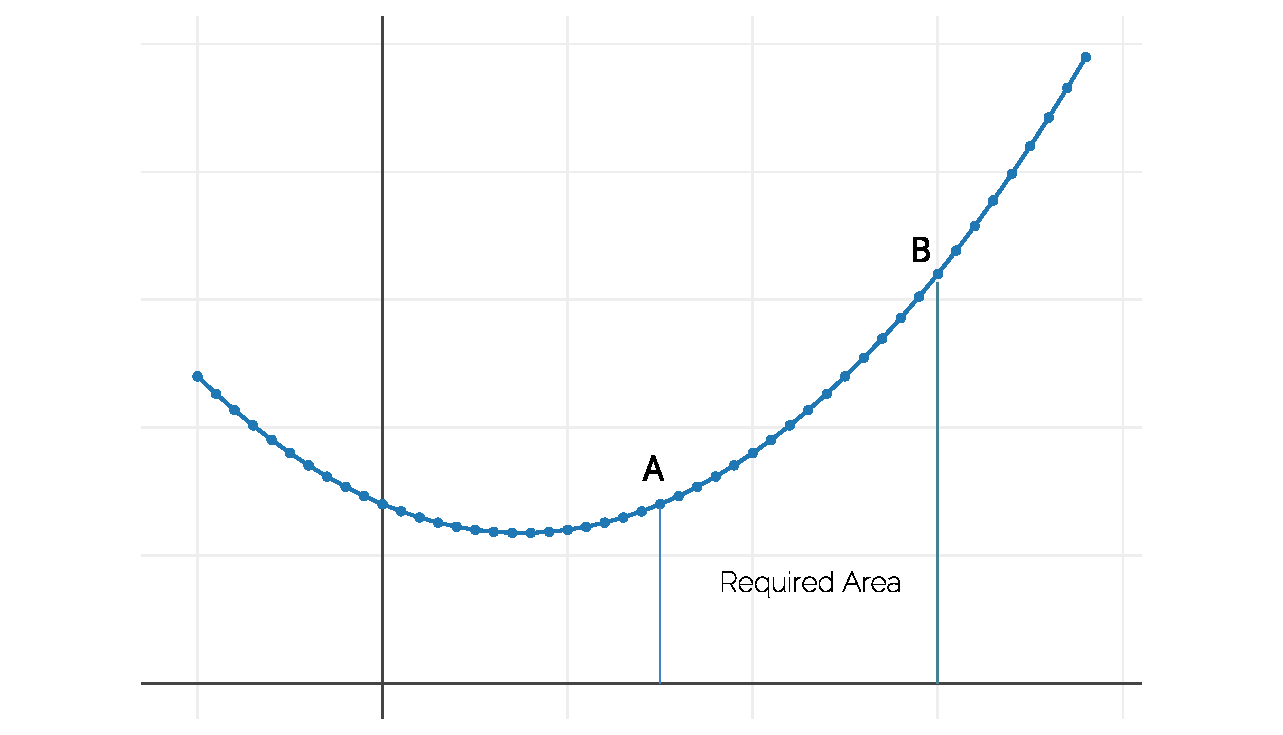
\includegraphics[width=300pt]{plotly.eps}
\fi

\begin{solution}[\halfpage]
	The required area $(R)$ is of the region between points $A$ and $B$ in the figure above.  

  \begin{align}
    R &= \int_{\vd}^{\ve} (\va x^2-\vb x+\vc)\ud x \\
      &= \left[ \va\cdot\dfrac{x^3}{3}-\dfrac{\vb}{2}x^2+\vc x\right]_{\vd}^{\ve} = \vf
  \end{align}
\end{solution}

\ifprintanswers
  \begin{codex}
    $\vf$ 
  \end{codex}
\fi
